% Document setup
\documentclass[12pt]{article}
\usepackage[margin=1in]{geometry}
\usepackage{fancyhdr}
\usepackage{lastpage}

\pagestyle{fancy}
\lhead{Richard Whitehill}
\chead{PHYS 804 -- HW \HWnum}
\rhead{\duedate}
\cfoot{\thepage \hspace{1pt} of \pageref{LastPage}}

% Encoding
\usepackage[utf8]{inputenc}
\usepackage[T1]{fontenc}

% Math/Physics Packages
\usepackage{amsmath}
\usepackage{amssymb}
\usepackage{mathtools}
\usepackage{physics}
\usepackage{siunitx}

\AtBeginDocument{\RenewCommandCopy\qty\SI}

% Enumeration/itemize
\usepackage{enumitem}
\newenvironment{parts}
{\begin{enumerate}[label=\textbf{(\alph*)},leftmargin=*,itemsep=-10pt]
}{\end{enumerate}}

% Reference Style
\usepackage{hyperref}
\hypersetup{
    colorlinks=true,
    linkcolor=blue,
    filecolor=magenta,
    urlcolor=cyan,
    citecolor=green
}

\newcommand{\eref}[1]{Eq.~(\ref{eq:#1})}
\newcommand{\erefs}[2]{Eqs.~(\ref{eq:#1})--(\ref{eq:#2})}

\newcommand{\fref}[1]{Fig.~\ref{fig:#1}}
\newcommand{\frefs}[2]{Figs.~\ref{fig:#1}--\ref{fig:#2}}

\newcommand{\tref}[1]{Table~\ref{tab:#1}}
\newcommand{\trefs}[2]{Tables~\ref{tab:#1}-\ref{tab:#2}}

% Figures and Tables 
\usepackage{graphicx}
\usepackage{float}
\usepackage[font=small,labelfont=bf]{caption}

\newcommand{\bef}{\begin{figure}[h!]\begin{center}}
\newcommand{\eef}{\end{center}\end{figure}}

\newcommand{\bet}{\begin{table}[h!]\begin{center}}
\newcommand{\eet}{\end{center}\end{table}}

% tikz
\usepackage{tikz}
\usetikzlibrary{calc}
\usetikzlibrary{decorations.pathmorphing}
\usetikzlibrary{decorations.markings}
\usetikzlibrary{arrows.meta}
\usetikzlibrary{positioning}
\usetikzlibrary{3d}
\usetikzlibrary{shapes.geometric}

% tcolorbox
\usepackage[most]{tcolorbox}
\usepackage{xcolor}
\usepackage{xifthen}
\usepackage{parskip}

\newcommand*{\eqbox}{\tcboxmath[
    enhanced,
    colback=black!10!white,
    colframe=black,
    sharp corners,
    size=fbox,
    boxsep=8pt,
    boxrule=1pt
]}

% problem-solution macros
% \usepackage{adjustbox}
\usepackage{changepage}

\newtcolorbox{probbox}[1][]{
    breakable,
    enhanced,
    boxrule=0pt,
    frame hidden,
    borderline west={4pt}{0pt}{green!50!black},
    colback=green!5,
    before upper=\textbf{Problem #1) \,},
    % \textbf{Problem #1 \ifthenelse{\isempty{#1}}{}{: #1} \\ },
    sharp corners,
    parbox=false
}

% \newtcolorbox{ProblemBox}[1][]{%
%   breakable,
%   enhanced,
%   colback=black!10!white,
%   colframe=black,
%   title={\large #1 \hfill}
% }
\newcommand{\prob}[2]{
\begin{probbox}[#1]
#2
\end{probbox}
}

\newenvironment{solution}{\begin{adjustwidth}{8pt}{8pt}}{\end{adjustwidth}}
\newcommand{\sol}[1]{
\begin{solution}
#1
\end{solution}
}
% \textbf{#1)} #2}

% Miscellaneous Definitions/Settings
\newcommand{\reals}{\mathbb{R}}
\newcommand{\integers}{\mathbb{Z}}
\newcommand{\naturals}{\mathbb{N}}
\newcommand{\rationals}{\mathbb{Q}}
\newcommand{\complexs}{\mathbb{C}}

\setlength{\parskip}{\baselineskip}
\setlength{\parindent}{0pt}
\setlength{\headheight}{14.49998pt}
\addtolength{\topmargin}{-2.49998pt}


\def\HWnum{3}
\def\duedate{October 5, 2024}

\begin{document}

\prob{1}{

A set of three integrals for testing numerical integration:
\begin{align}
    \int_{0}^{1} x^3 \dd{x} = \frac{1}{4}, \quad \int_{0}^{1} e^{x} \dd{x} = e - 1, \quad \int_{0}^{\pi} \sin{x} \dd{x} = 2
.\end{align}

\begin{parts}

    \item Write a program (that will be your code 1) that calculates an integral with a given integrand $f(x)$ in the region $[a,b]$ by one of the Newton-Cotes rules with $n \geq 1$ (the trapezoid rule, or 3-point Simpson's rule, or 5-point Boole's rule or higher) and test it on the set of three ``test'' integrals.
        Explore how the accuracy changes with the number of integrals.

    \item Upgrade/modify your code (that will be your code 2) to include the error estimate based on calculations for two step sizes $h$ and $h/2$.
        You can find the error estimation in the lecture notes (see ``Extrapolation and Romberg integration'').
        Test your code with the set of three test integrals.
        Now you have a tool to estimate accuracy of numerical integration.

    \item Write a program (that will be your code 3) that calculates an integral from $f(x)$ in the region $[a,b]$ by using Gauss quadratures for 10 points.
        Coefficients for Gauss quadratures can be found in Abramowitz and Tegun ``Handbook of Mathematical Functions'', or on the web.
        Again, test your code with the three test integrals.

    \item Find an integration routine (preferably adaptive) you can use with the language of your choice (Python, C$++$, or MatLab).
        That will be your code 4.
        Again, test your routine with the three test integrals.
    
\end{parts}

}

\sol{

(a) In general, we would like to approximate the integral
\begin{align}
    I = \int_{a}^{b} f(x) \dd{x}
,\end{align}
which can be done as a weighted sum
\begin{align}
    I \approx \sum_{i} w_i f(x_{i})
.\end{align}
Of course, it befalls us to choose a good set of $x_{i}$ and weights $w_{i}$ in order to obtain a good approximation for $I$.
A generic Newton-Cotes integration rule is derived by approximating the function $f(x)$ over the integration domain with an interpolating polynomial $L(x)$:
\begin{align}
    I = \int_{a}^{b} f(x) \dd{x} \approx \int_{a}^{b} L(x) \dd{x}
.\end{align}
In the Lagrange interpolation scheme, if we have a set of sample points $\{ (x_0,f(x_0)),\ldots,\\ (x_{n},f(x_{n})) \}$, we can interpolate $f(x)$ with an $n^{\rm th}$ order polynomial
\begin{align}
    L(x) = \sum_{i=0}^{n} f(x_{i}) l_{i}(x)
,\end{align}
where $\{l_{i}(x)\}$ is the interpolating basis and $l_{i}(x_{j}) = \delta_{ij}$.
Thus, with the Newton-Cotes scheme
\begin{align}
    I \approx \sum_{i=0}^{n} f(x_{i}) \int_{a}^{b} l_{i}(x) \dd{x}
.\end{align}
Thus, the weights are just the integrals of the interpolating polynomials.
For this work, we implement the simplest Newton-Cotes rule, which is equivalent to the trapezoid rule.
We first break the integration region into $N$ intervals, giving us a sub-interval width $h = (b - a) / N$ and $N+1$ sample points $\{ a=x_0,\ldots,x_{i},x_{i+1},\ldots,x_{N}=b \}$.
Using a simple linear interpolation for the sub-interval $[x_{i},x_{i+1}]$, our Lagrange basis is
\begin{align}
    l_{1}(x) = \frac{x - x_{i+1}}{x_{i} - x_{i+1}} = -\frac{x - x_{i+1}}{h}, \quad l_{2}(x) = \frac{x - x_{i}}{h}
,\end{align}
and
\begin{align}
    \int_{x_{i}}^{x_{i+1}} l_{1}(x) \dd{x} = -\frac{(x - x_{i+1})^2}{h} \Big|_{x_{i}}^{x_{i+1}} = \frac{h}{2} \\
    \int_{x_{i}}^{x_{i+1}} l_{2}(x) \dd{x} = \frac{(x - x_{i})^2}{h} \Big|_{x_{i}}^{x_{i+1}} = \frac{h}{2}
.\end{align}
Thus, over the sub-interval $[x_{i},x_{i+1}]$
\begin{align}
    \int_{x_{i}}^{x_{i+1}} f(x) \dd{x} \approx \frac{h}{2} ( f(x_{i+1}) + f(x_{i}) )
.\end{align}
If we now sum over all the sub-intervals, we find
\begin{align}
    \int_{a}^{b} f(x) \dd{x} &= \sum_{i=0}^{N} \int_{x_{i}}^{x_{i+1}} f(x) \dd{x} \approx \frac{h}{2} \sum_{i=0}^{N} [ f(x_{i}) + f(x_{i+1}) ] \nonumber \\
                             &= \frac{h}{2}[ f(x_{0}) + 2 f(x_{1}) + \ldots + 2 f(x_{n-1}) + f(x_{n}) ]
.\end{align}
Results using the Trapezoidal integration are shown in \fref{prob1}.


(b) Romberg integration is a method which uses the following motivation.
Let us denote our approximate integral, which is a function of the step-size $h$ of our sub-intervals, as $I(h)$, where the exact result
\begin{align}
    I = I(h) + \sum_{k=0}^{\infty} a_{k} h^{n+km}
,\end{align}
where $n,m$ are some integers.
In particular, if we compute our integral at two step-sizes $h$ and $h/N$, we have
\begin{align}
    I &= I(h) + a_0 h^{n} + \sum_{k=1}^{\infty} a_{k} h^{n+km} \\
    I &= I(h/N) + a_0 (h/N)^{n} + \sum_{k=1}^{\infty} a_{k} (h/N)^{n+km}
.\end{align}
We then have
\begin{align}
    0 = I(h) - I(h/N) + a_0 h^{n} \Big( 1 - \frac{1}{N^{n}} \Big) \Rightarrow a_0 h^{n} = \frac{N^{n}}{N^{n} - 1} \Big[ I(h/N) - I(h) \Big]
,\end{align}
where we have neglected $\mathcal{O}(h^{n+m})$ terms.
This is effectively gives us an estimate of our trapezoidal integrations and an extrapolated value for the integral
\begin{align}
    I \approx I(h/N) + a_0 (h/N)^{n} = I(h/N) + \frac{1}{N^{n} - 1} \Big[ I(h/N) - I(h) \Big]
.\end{align}
Results using the Trapezoidal integration are shown in \fref{prob1}.


(c) We now discuss Gauss-Legendre quadrature.
First, we make the change of variables $x = \frac{b-a}{2} t + \frac{a+b}{2}$ such that
\begin{align}
    I = \int_{a}^{b} f(x) \dd{x} = \int_{-1}^{1} \frac{b-a}{2} f(x(t)) \dd{t}
.\end{align}
Again, we would like to find suitable weights and sample points $\{ (w_{i},x_{i}) \}$ such that
\begin{align}
    I \approx \sum_{i=1}^{n} w_{i} f(x_{i})
.\end{align}
Our inspiration here is the Taylor expansion
\begin{align}
    f(x(t)) = \sum_{n=0}^{2N-1} a_{n} t^{n} + \mathcal{O}(t^{2N}) \approx p_{2N-1}(t)
,\end{align}
over the interval $[-1,1]$.
At this point, we would like to define our weights and sample points such that 
\begin{align}
    \int_{-1}^{1} p_{2N-1}(t) \dd{t} = \sum_{i=1}^{N} w_{i} p_{2N-1}(t_{i})
.\end{align}
Following through, we have
\begin{gather}
    \sum_{n=0}^{2N-1} a_{n} \frac{1 - (-1)^{n+1}}{n+1} = \sum_{i=0}^{N} w_{i} \sum_{n=0}^{2N-1} a_{n} t_{i}^{n} \Rightarrow
    \sum_{i=1}^{N} w_{i} t_{i}^{n} = \frac{1 + (-1)^{n}}{n+1}
\end{gather}
for all $n \in \{0,\ldots,2N-1\}$.
We thus have $2N$ -- not necessarily linear -- equations for $2N$ unknowns.
Let us solve this for a the simplest case of $N = 1$.
First, for $N = 1$, we have only two equations
\begin{align}
    \begin{cases}
        w_1 + w_2 = 2 \\
        w_1 t_1 + w_2 t_2 = 0 \\
        \displaystyle w_1 t_1^2 + w_2 t_2^2 = \frac{2}{3} \\
        w_1 t_1^3 + w_2 t_2^3 = 0
    .\end{cases}
\end{align}
Carrying out the algebra, one finds $w_{1} = w_{2} = 1$ and $t_{1} = -t_{2} = 1/\sqrt{3}$.
One could continue producing weights and sample points for larger $N$, but it turns out that we can be a little bit more clever in how we determine them.
While the details are beyond the scope of this report, we can choose our points $t_{i}$ such that they are roots of the $N^{\rm th}$ Legendre polynomial, $P_{N}(t)$.
That is $P_{N}(t_{i}) = 0$.
These roots have several nice properties, including that they are symmetrically distributed about $t = 0$ and all distinct.
The corresponding weights are given by
\begin{align}
    w_{i} = \frac{2}{(1 - t_{i}^2) [P_{N}'(t_{i})]^2}
.\end{align}
These weights and roots are tabulated within the \textit{numpy} library, and as such, we can pulled up to an arbitrarily large $N$.
Before concluding, it should be noted that the sucess of this method depends on the behavior of our integrand.
That is, our function and its derivatives should be reasonably smooth in order to be well approximated by a sufficiently low-order polynomial over the integration range of interest.
Results using the fixed-order Gaussian quadrature discussed here is shown in \fref{prob1}.

(d) The \textit{scipy.integrate} module provides a generic adaptive integration routine \textit{quad}.
We use this to benchmark our other quadrature implementations.
Results using this function are shown in \fref{prob1}.


The code below implements all the essential quadrature algorithms.
\inputpython{main.py}


\begin{figure}[h!tb]
    \centering
    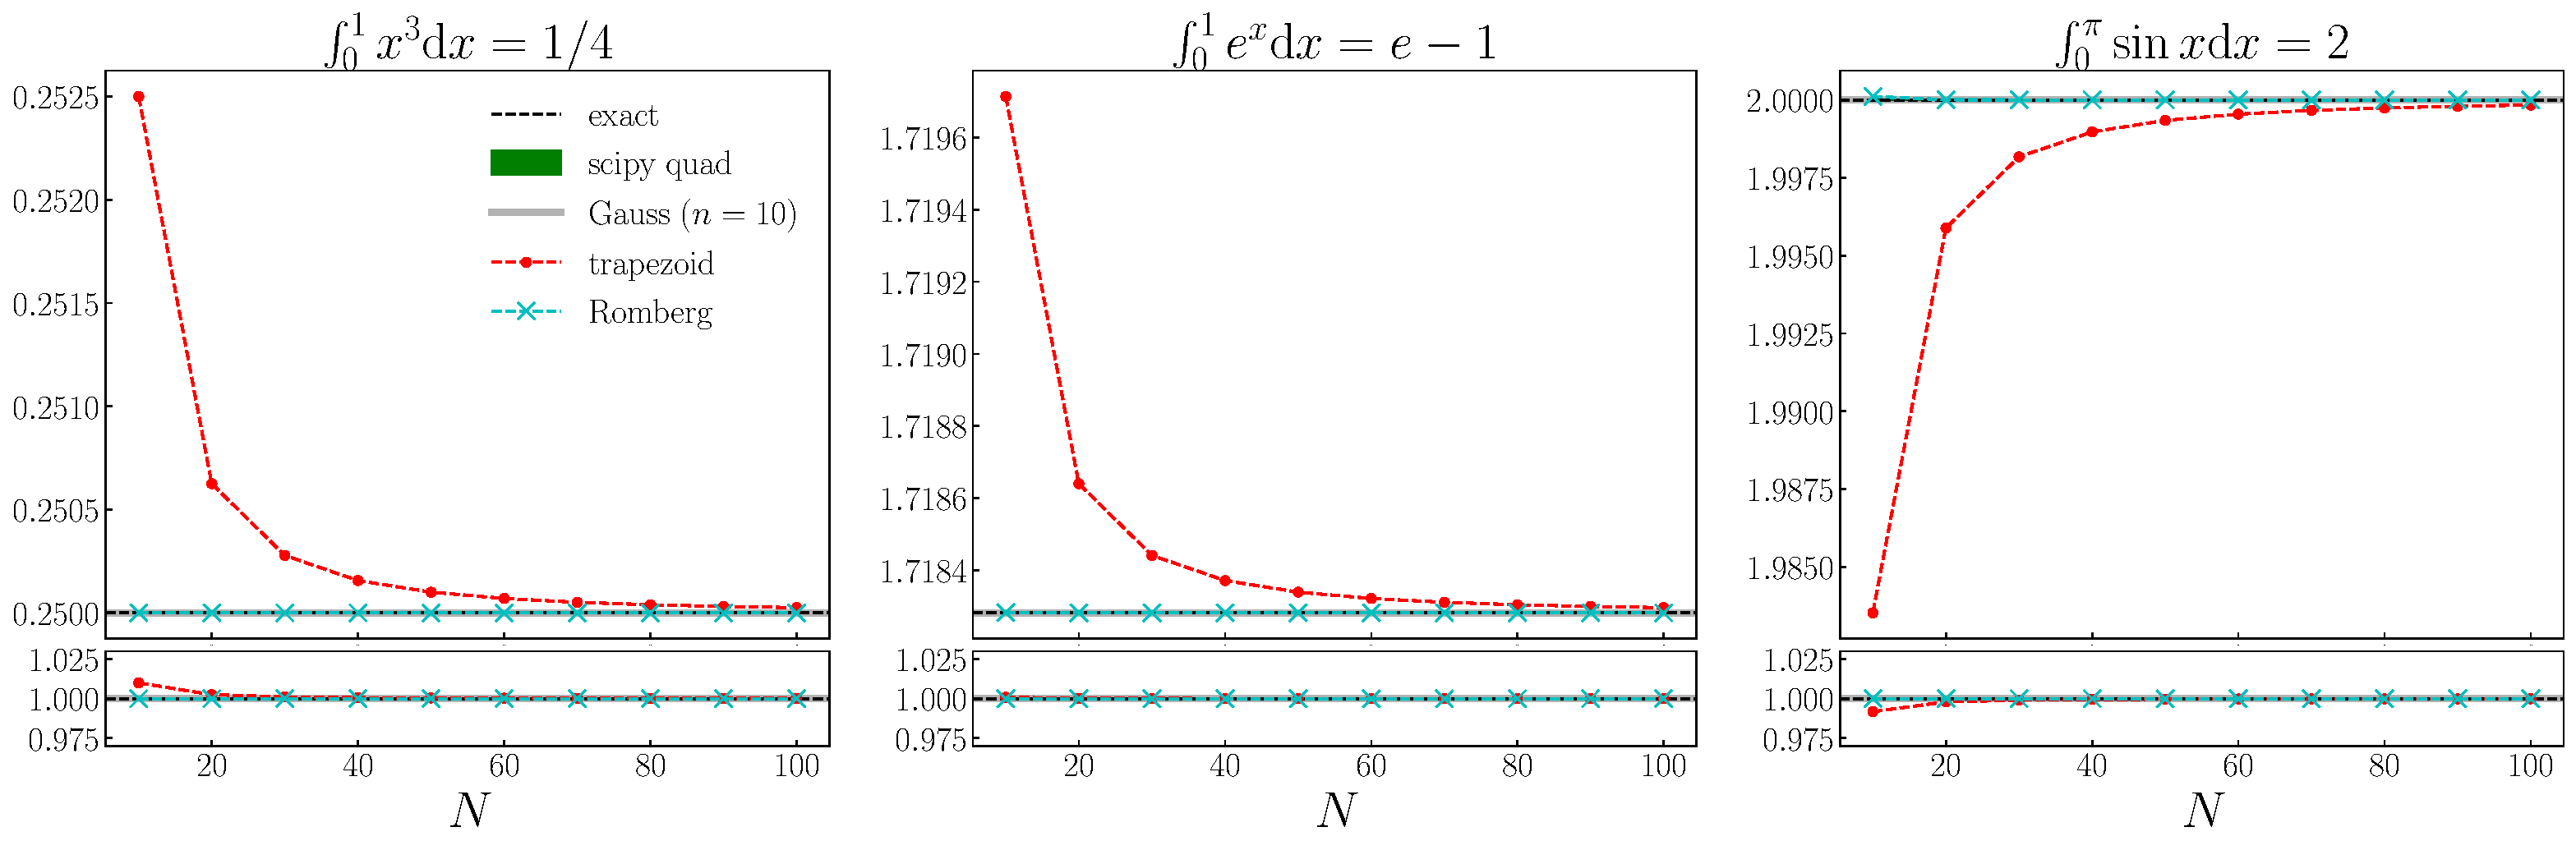
\includegraphics[width=\textwidth]{prob1.pdf}
    \caption{Results for the various quadrature routines discussed in this problem. The top row of panels displays the trapezoidal and Romberg integrations as functions of the number of intervals against the fixed-order Gaussian quadrature, \textit{quad}, and exact results, and the bottom row of panels displays the ratio of each implemented method relative to the exact result.}
    \label{fig:prob1}
\end{figure}


}


\prob{2}{

Evaluate the following integrals using your codes 2, 3, and 4:
\begin{parts}
   
\item $\displaystyle \int_{0}^{1} \frac{1}{1-0.998 x^2} \dd{x}$

\item $\displaystyle \int_{0}^{2\pi} x \sin(30 x) \cos(50 x)$
    
\item $\displaystyle \int_{0}^{1} \frac{x}{e^{x} - 1} \dd{x}$

\item $\displaystyle \int_{0}^{1} x \sin(\frac{1}{x}) \dd{x}$

\end{parts}

Report if one of your codes fails to compute some of the integrals.
Explain why.

}

\sol{

The results are shown in \tref{prob2}.
Most of the non-adaptive codes implemented in problem 1 fail to produce an accurate result across each integral here.

(a) The integrand has a singularity at $x = 1/\sqrt{0.998} \approx 1.001$ and is therefore very steep in this region.
Thus, we would need a large number of sub-intervals to accurately capture the behavior in this region.
Additionally, this function requires many terms in the Taylor expansion to accurately capture the behavior as $x \rightarrow 1$, meaning that while the Gaussian quadrature performs better than the Trapezoidal integration on the same number of function evaluations, we should crank up $n$ in order to more accurately calculate the area under the curve.

(b) The integrand here oscillates very rapidly over the region of interest, making the quadrature routines fairly unstable for small numbers of function evaluations.
While not done here, it would not be difficult to split the integration region between the integrand's zeros, apply the quadrature routines on these sub-intervals, and sum each contribution.
This is the typical advice for periodic functions.
It can be seen especially that the performance of the Gaussian quadrature implementation becomes much more accurate with a relatively small $n$ on each sub-interval.

(c) Observe that
\begin{align}
    \frac{x}{e^{x} - 1} \rightarrow 1 - \frac{x}{2} + \ldots
\end{align}
as $x \rightarrow 0$, so in this case, instead of a singularity at $x = 0$ we have some indeterminacy.
Of course, though, naively applying trapezoidal and Romberg integration on the provided integration domain provides non-finite results since we evaluate at exactly $x = 0$ and returns $0/0$ even though our function is finite throughout the integration domain.
In practice, we could amend these issues by providing an alternate definition of our function such that at $x = 0$, we return $1$, filling in the point discontinuity that is formally there.

With Gaussian integration, we avoid this subtle business since there is no function evaluation at the end points and obtain reasonably accurate results with a small number of function evaluations.


(d) The discussion here is similar to that of parts (b) and (c).
Observe that our function is formally undefined at $x = 0$, but this discontinuity is simply a hole that could be filled by redefining our function to take the limiting value at $x \rightarrow 0$.
Additionally, we can observe that our function oscillates rapidly in this limit, and even if this oscillation is not periodic, we can analytically determine the location of the integrand's roots, which would allow us to simply split our integration domain (although this is not done here).
It turns out that fixed-order Gaussian integration and adaptive integration do a reasonably good job of providing an accurate value for this integral.

\begin{table}[h!tb]
    \centering
    \begin{tabular}{|c||c|c|c|c|}
        \hline
        Part & Trapezoid ($N = 100$) & Romberg ($N = 100$, R=2) & Gauss ($n = 10$) & \textit{scipy} \\
        \hline
        a & 5.362 & 4.633 & 3.175 & 3.804 \\
        b & 0.272 & 0.319 & 3.303 & 0.112 \\
        c & nan & nan & 0.778 & 0.778 \\
        d & nan & nan & 0.387 & 0.379 \\
        \hline
    \end{tabular}
    \caption{Results of quadrature routines applied to the integrals specified.}
    \label{tab:prob2}
\end{table}


\inputpython{prob2.py}

}


\prob{3}{

Evaluate numerically following improper integrals (you may need to modify one of your codes).
There are multiple ways to evaluate improper integrals.
Explain your choice and results.
\begin{parts}

\item $\displaystyle \int_{0}^{\infty} \frac{e^{-x^2}}{x^2 + 1} \dd{x}$

\item $\displaystyle \int_{0}^{\infty} \frac{x \sin{x}}{x^2 + 1} \dd{x}$

\item $\displaystyle \int_{0}^{\infty} e^{-\sqrt{x}} \cos(2x) \dd{x}$
    
\end{parts}

}

\sol{

While there are nicer methods to handle improper integrals such as these, we can make a simple substitution to map our infinite domain of integration onto a finite domain:
\begin{align}
    x = \tan{u} \Rightarrow \int_{a}^{b} f(x) \dd{x} = \int_{\arctan(a)}^{\arctan(b)} \frac{f(\tan{u})}{\cos^2{u}} \dd{u}
.\end{align}
Notice that if $a = \infty$, then $\arctan{a} = \pi/2$, or if $b = -\infty$, then $\arctan{b} = -\pi/2$.
With this, we can employ the integration techniques from Problem 1 with some caveats.
Results are shown in \tref{prob3}.
While our fixed-order integration provides reasonably accurate results for the integrals of parts (a) and (c), it fails to do so for part (b)'s integral, primarly because of the oscillation.
For these kinds of integrals, it may be best to simply observe that this function dies off as $1/x$ as $x \rightarrow \infty$ and integrate over successive intervals (defined by the roots of the integrand) until some specified tolerance is achieved since over each such interval, our function is well-behaved.

\begin{table}[h!tb]
    \centering
    \begin{tabular}{|c||c|c|}
        \hline
        Part & Fixed Gauss & \textit{scipy} \\
        \hline
        a & 0.672 ($n = 10$) & 0.672 \\
        b & -2.11 ($n = 10$) & 1.255 \\
        c & 0.122 ($n = 1000$) & 0.123 \\
        \hline
    \end{tabular}
    \caption{Results of a modified fixed-order Gaussian quadrature routine and adaptive quadrature applied to the integrals specified above.}
    \label{}
\end{table}

\inputpython{prob3.py}

}


\prob{4}{

Evaluate numerically following principal value integrals using one of techniques for princpal value integrals (again, you may need to modify one of your codes).

\begin{parts}

\item $\displaystyle \int_{0}^{1} \frac{1}{x^{1/3}} \dd{x}$

\item $\displaystyle \int_{-1}^{1} \Big( 1 + \frac{1}{x} \Big) \dd{x}$

\item $\displaystyle \int_{-\infty}^{\infty} \frac{1}{(x - 1)(x^2 + 1)} \dd{x}$
    
\end{parts}

}

\sol{

(a) We can employ Gaussian quadrature directly on the integral here since our troubles are only at the endpoint $x = 0$ but the routines never evaluate there.
It is observed that our routines are quite accurate here.

(b) Unlike in part (a), since our integral has difficulties around $x = 0$, we split explicitly the integration domain into two sub-intervals $[-1,0] \cup [0,1]$.
Doing so analytically, it is simple to see that the pathological piece $1/x$ cancels in the principal value prescription since it is odd about $x = 0$, and because of this, our integration routines are quite accurate.

(c) This integral can be performed analytically by utilizing partial fraction expansion.
It is a simple matter then to see that the singular piece cancels in the principal value prescription, leaving us with a finite Lorentzian.
It is interesting to note that fixed-order Gaussian integration performs quite well for part (c) but the \textit{quad} function requires large but not infinite (\textit{np.inf}) bounds to be inserted.
In the code shown below, we replace the bounds with $\pm 100$.


The results are as follows
\begin{table}[h!tb]
    \centering
    \begin{tabular}{|c||c|c|c|}
        \hline
        Part & Fixed Gauss & \textit{scipy} & exact \\
        \hline
        a & 1.499 ($n = 100$) & 1.5 & 1.5 \\
        b & 2.0 ($n = 10$) & 2.0 & 2 \\
        c & $-1.021$ ($n = 100$) & $-1.571$ & $-\pi/2$ \\
        \hline
    \end{tabular}
\end{table}


\inputpython{prob4.py}

}


\prob{5}{

Evaluate numerically following double integrals.
\begin{parts}

\item $\displaystyle \int_{-1}^{1} \dd{x} \int_{0}^{2} \dd{y} \sin(x^2 + y^2)$

\item $\displaystyle \int_{0}^{1} \dd{x} \int_{0}^{1-x} \dd{y} \frac{1}{\sqrt{x + y} (1 + x + y)^2}$
    
\end{parts}


}

\sol{

For these multi-dimensional integrations, we utilize the iterative intregration scheme.
That is, our integral of interest is
\begin{align}
    I = \int_{a}^{b} \dd{x} \int_{y_1(x)}^{y_2(x)} \dd{y} f(x,y) = \int_{a}^{b} \dd{x} F(x)
,\end{align}
where 
\begin{align}
    F(x) = \int_{y_1(x)}^{y_2(x)} \dd{y} f(x,y)
.\end{align}
Now we can set up $F(x)$ as a function, which employs one integration over the variable $y$ at a given $x$, and set up a second integration of $F(x)$.
While Gaussian quadrature performs nicer than Monte Carlo integration in one dimension over a large set of functions, one can appreciate here the utility of Monte Carlo methods for higher-dimensional integrations.
If one uses Gaussian quadrature with $n$ points for each integration dimension, then in total we will require $n^D$ points for an integral over $D$ variables, which is exponentially poor.
However, as we have learned previously, if we sample the integrand, we may hope to reduce the number of points needed to evaluate the integral.

(a) Using the iterated integral presription above and the fixed-order Gaussian quadrature from problem (1), we obtain
\begin{align}
    I \approx 1.753
,\end{align}
which is quite accurate since our function is well-behaved over the integration domain.

(b) Using the iterated integral prescription above and the adaptive quadrature function from \textit{scipy}, we obtain
\begin{align}
    I \approx 0.285
.\end{align}
Note that we required adaptive quadrature since there is a singularity at the origin.


\inputpython{prob5.py}

}


\prob{6}{

Write a program that employs either adaptive or automatic numerical integration.
Appy your code to integrals in part 2.

}

\sol{

We implement a simple adaptive routine via recursion.
That is, we first compute the integral
\begin{align}
    I_1 = \int_{a}^{b} f(x) \dd{x}
\end{align}
and the two integrals
\begin{align}
    I_2 = \int_{a}^{(a+b)/2} f(x) \dd{x} + \int_{(a+b)/2}^{b} f(x) \dd{x}
.\end{align}
If the relative and absolute difference between these two integrals are within prescribed tolerances we return $I_2$.
Otherwise, we further split the integration domains of each integration and repeat the conditional checks until they are satisfied or the maximum recursion depth is achieved.
The results of implementing this method with fixed Gaussian quadrature as our base function are shown in the following table.
It can be see that they match reasonably with our results from problem 2 obtained with the \textit{scipy} adaptive routine.
\begin{table}[h!tb]
    \centering
    \begin{tabular}{|c||c|}
        \hline
        Part & Adaptive Gauss ($n = 100$) \\
        \hline
        a & 3.804 \\
        b & 0.118 \\
        c & 0.778 \\
        d & 0.379 \\
        \hline
    \end{tabular}
\end{table}


\inputpython{prob6.py}

}



    
\end{document}
